\documentclass[a4paper,10pt]{article}
\usepackage[utf8]{inputenc}
\usepackage{graphicx}
\usepackage{amsmath}
\usepackage{gensymb}
\usepackage{makeidx}
\usepackage{hyperref}

\hypersetup{colorlinks=true,linkcolor=blue,urlcolor=blue}

%opening
\title{The Ellipses}
\author{Francesco Lazzarotto (INAF Padova)\\ francesco.lazzarotto@inaf.it}

\begin{document}

\maketitle

\begin{abstract}
An ellipse, defined in a 2D plane X, Y is a closed, smooth oval curve defined as the set of all points in a plane where the sum of the distances to two fixed points ($F_1, F_2$), is constant, that points called foci (plural of focus). In figure \ref{ellipse1} you can see that for each point P(x,y), the sum of the distances from it and $F_1$ ($L_1$) and from it and $F_2$ ($L_2$) is constant: \(L_1 + L_2 = k\). The ellipse in \ref{ellipse1} has it's center in the origin of the cartesian axes, it has the major axes on the X axes and the minor axes on the Y axes. The minor semiaxes is defined to have $b$ length, while the major semiaxes is defined to have $a$ length. The distance of the foci from the center is defined of length $c$, with \(c = \sqrt{a^2-b^2} \). The points \( ( \pm c,0) \) called foci. are extremely important in \emph{Astronomy}, since celestial objects, included planets, follow elliptical orbits with the sun at a focus, not with the sun at the center. The points $(\pm a,0)$ and $(0, \pm b)$) are called vertices. If $ a > b > 0 $, then the major axis is the line segment from (-a,0) to (a,0) and the semi-major axis is the line segment from the origin to (a,0).
Likewise, the minor axis runs from (0,-b) to (0,b) and the semi-minor axis runs from the origin to (0,b).
If $b > a > 0$, then the major and semi-major axes are vertical and the minor and semi-minor axes are horizontal.
We wiil show first the case where $a>b$, that the ellipse is ``short and fat''.
The ellipse is also a \emph{conic section} formed by intersecting a cone with an angled plane, representing a stretched circle.
\end{abstract}
\tableofcontents
\newpage
\begin{figure}[!ht]
\begin{center}
 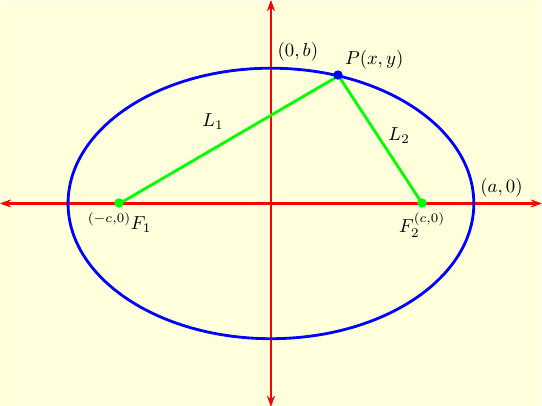
\includegraphics[width=10cm]{ellipse_foci.png}
\end{center}
\caption{Ellipse with foci}
\label{ellipse1}
\end{figure}
\begin{figure}[!ht]
\clearpage
\begin{center}
 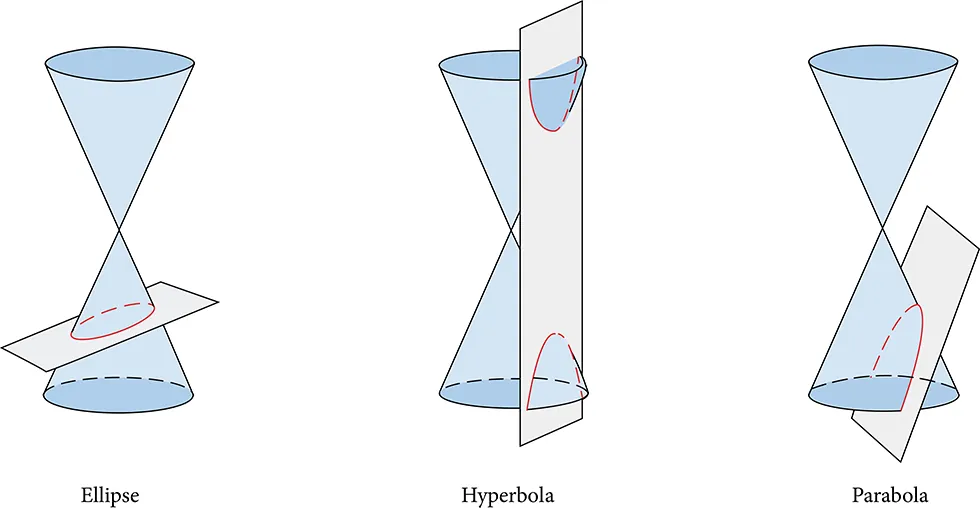
\includegraphics[width=10cm]{conics.png}
\end{center}
\caption{Conic sections}
\label{conics1}
\end{figure}
\section{Introduction}
In the next sections we will use the assumption that the ellipse has the center in (0,0), the center of the cartesian reference OXY.
Here a mathematical description of ellipses in the 2D plane, including definitions, equations, parametric equations, foci, semiaxes, eccentricity, area, perimeter (approximation), arcs, translation, and rotation. We will also provide a C program that demonstrates some of these concepts and generates data for plotting an ellipse using gnuplot \cite{gnuplotJ16} .\\
Steps:\\
\begin{enumerate}
\item general introduction
\item Definition of an Ellipse
\item Standard Equation of an Ellipse
\item Parametric Equations
\item Foci and Eccentricity
\item Semiaxes
\item Area and Perimeter (Approximation)
\item Arcs and Sector Area (Approximation)
\item Translation of Ellipse
\item Rotation of Ellipse
\item Example with C Code and gnuplot
\end{enumerate}
\subsection{Conics}
A conic section, or just conic, is a shape resulting from intersecting a right circular cone with a plane. The angle at which the plane intersects the cone determines the shape, as shown in Figure \ref{conics1} .\\
\subsection{Cartesian Equation}
The ellipse can be described via Cartesian (rectangular) coordinates by the following equation.
\[  \frac{x^2}{a^2}+\frac{y^2}{b^2}=1. \]
This formula is based on distance and defines the "static" shape.
\begin{itemize}
 \item a = horizontal semi-axes
 \item b = vertical semi-axes
\end{itemize}
How do you use it? It's perfect for instantly seeing where the ellipse intersects the axes and for checking whether a point is on the edge, inside, or outside the curve.
\subsection{Eccentricity}
\begin{figure}[!ht]
\begin{center}
 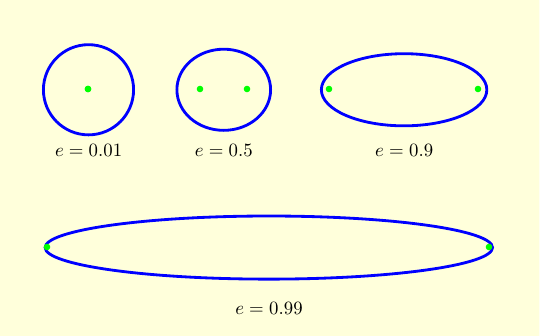
\includegraphics[width=12cm]{ellipses_ecc.png}
\end{center}
\caption{Ellipses with different eccentricity}
\label{eccentr}
\end{figure}
The ratio $c/a$ is called the \emph{eccentricity} of the ellipse, and is usually denoted e. Note that \(0 \leq e<1 \). A circle can be viewed as an ellipse with eccentricity zero, and with both foci coincident in the origin. You can see ellipses of different eccentricity in figure \ref{eccentr} .
\subsection{Parametric equations}
It is possible to define an ellipse as a parametrized curve, taking
\[
\begin{cases}
x=a\cos(t)\\
y=b\sin(t)
\end{cases}
\]
with the parameter (angle) t running from 0 to \( 2\pi \).
How do you use it? It's the standard format for graphics and animation software. If you want to make an object move along an elliptical path, you use these formulas to calculate its position instant by instant.
What is the difference between a cartesian equation and a parametric equation?
The main difference lies in how they describe the shape (line, plane, or curve). Here's a quick comparison:
\begin{enumerate}
\item Cartesian Equation\\
Relates coordinates (x,y,z) directly. It tells you whether a point belongs to the shape by "testing" its coordinates.
\begin{itemize}
\item Shape: A single equation (e.g., for a straight line in the plane: $ ax + by + c $ ).
\item Example: $ y = 2x + 1 $
\item Advantage: It's easy to understand the relationship between variables (e.g., the slope) and verify whether a point is "inside" or "outside."
\item Disadvantage: It becomes complicated for shapes that are not functions (like circles, where $ x^2 + y^2 = r^2 $ is needed, and ellipses as well).
\end{itemize}
\item Parametric Equation\\
Expresses each coordinate as a function of an external variable called a parameter (usually t ).
\begin{itemize}
\item Form: A system of equations (one for each dimension).
\item Example:
\begin{itemize}
\item $ x = t $
\item $ y = 2t + 1 $
\end{itemize}
\item Advantage: Describes motion. If you think of it as "time," the equation tells you where the object is at any given moment. It is essential in 3D graphics and physics.
\item Disadvantage: It is less intuitive for visualizing the overall shape at a glance.
\end{itemize}
\textbf{In summary}:
\begin{itemize}
\item Cartesian: It is like a static "picture." It defines the figure as the set of points that satisfy a rule.
\item Parametric: It is like a "movie." It gives you instructions for tracing the figure point by point at the changing of the parameter.
\end{itemize}
\end{enumerate}
\newpage
\subsection{Plotting an ellipse}
We will show here how to plot an ellipse with gnuplot \cite{gnuplotJ16} using parametric equations.\\
You must first enable parametric mode and then define the functions x and y based on the default variable t.
Here are the steps and the code to type in the gnuplot terminal or save in a source file:
\begin{enumerate}
\item Enable parametric mode: Use the set parametric command.
\item Set the aspect ratio: Use set size ratio -1 to ensure the axes have the same scale, otherwise the ellipse will appear distorted.
\item Define the parameters: Set the values for the semi-axes a (horizontal) and b (vertical).
\item Run the plot: Use the \verb|plot| command, providing the two functions separated by a comma.
\end{enumerate}
\begin{verbatim}
# 1. Environment configuration
set parametric
set size ratio -1
set grid

# 2. Shape Parameters definition (e.g.: a=5, b=3)
a = 5
b = 3

# 3. Set the interval of the t parameter (from 0 to 2*pi for a complete loop)

set trange [0:2*pi]

# 4. Plot the ellipse
plot a*cos(t), b*sin(t) title "Parametric Ellipse"
\end{verbatim}
\begin{figure}[!ht]
\begin{center}
 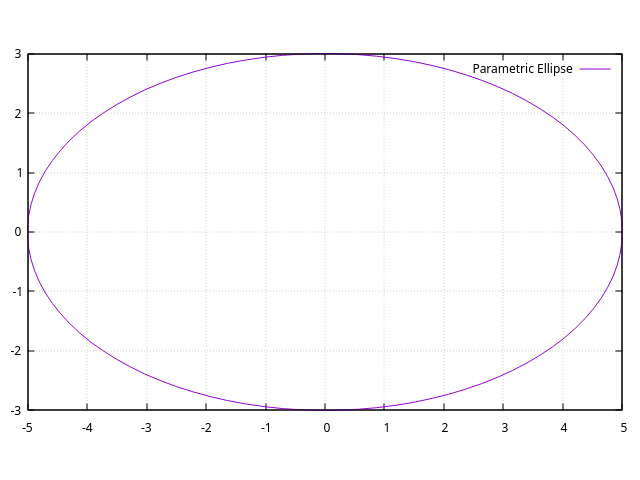
\includegraphics[width=12cm]{parellipse.png}
\end{center}
\caption{Ellipse plotted using parametric equations}
\label{ellipse2}
\end{figure}
save this code in a text file called \verb|parellipse.plt| and run it. If you open a terminal in the same folder of the file, you can plot the ellipse with the command
\begin{verbatim}
gnuplot -p parellipse.plt
\end{verbatim}
and press enter \verb|<--|
\subsubsection{Command Explanation}
\begin{itemize}
 \item \verb|set parametric|: Changes the behavior of the plot command. Instead of expecting $ y = f(x) $, gnuplot expects a pair of functions $ x(t), y(t) $ .
 \item t: This is the default dummy variable for 2D curves in parametric mode.
 \item  \verb|a*cos(t), b*sin(t)|: These are the standard parametric equations for the ellipse centered at the origin.
 \item \verb|set size ratio -1|: This is essential to ensure that one unit on the X-axis is equal to one unit on the Y-axis on the screen.
If you want to move the center of the ellipse to a point,
just change the plot command to:\\
\verb|plot h + a*cos(t), k + b*sin(t)|
\end{itemize}
Here in figure \ref{ellipse2} the graph result of the script shown here.
\newpage
\subsubsection{Plot a circle}
\begin{figure}[!ht]
\begin{center}
 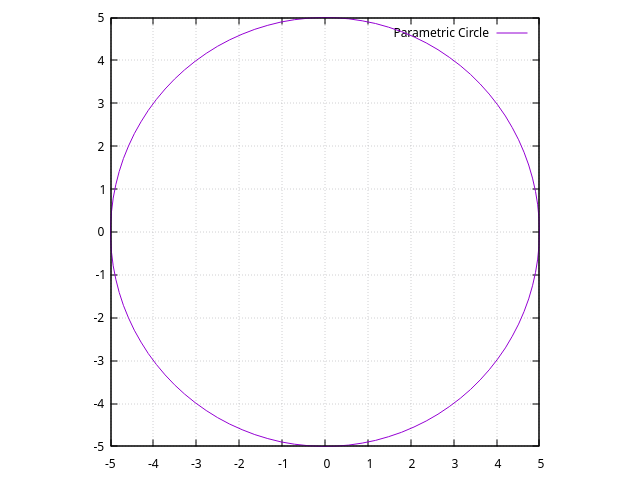
\includegraphics[width=10cm]{parcircle.png}
\end{center}
\caption{Circle plotted using parametric equations}
\label{circle1}
\end{figure}
To plot a circle using the same script we will modify accordingly the following lines of code
\begin{verbatim}
# 2. Shape Parameters definition (e.g.: a=5, b=5)
a = 5
b = 5
\end{verbatim}
So the ellipse with equal semi-axes will converge to a circle (figure \ref{circle1}). And then we'll run again the script with the same instruction.
\section{Mathematical description}
\subsection{Definition:}
\begin{quote}
    An ellipse is the set of points in a plane such that the sum of the distances from two fixed points (foci) is constant.
\end{quote}
\subsection{Standard Equation:}
For an ellipse centered at \((x_c, y_c)\) with semi-major axis a (horizontal) and semi-minor axis b (vertical) the following equation is valid:
      \[  \frac{(x - x_c)^2}{a^2} + \frac{(y - y_c)^2}{b^2} = 1 \]
    If the ellipse is oriented with the major axis vertical, then a and b swap roles.
\subsection{Parametric Equations:}
    \[ x = x_c + a \cdot cos(t) \]
    \[ y = y_c + b \cdot sin(t) \]
    where t is the parameter (usually from 0 to 2\(\pi\)).
\subsection{Foci and Eccentricity:}
    The foci are located at \((x_c \pm c, y_c)\) for a horizontal major axis,\\ where \(c = \sqrt{a^2 - b^2}\).\\
    Eccentricity \(e = \frac{c}{a}\,\,(0 \leq e < 1)\).\\
\subsection{Semiaxes:}
    a: semi-major axis (longer)\\
    b: semi-minor axis (shorter)\\
\subsection{Area and Perimeter:}
    Area = \( \pi \cdot a \cdot b \)\\
    Perimeter (approximation): There is no closed-form formula, but one approximation is:
       \[ P \approx \pi \cdot [ 3(a+b) - \sqrt{(3a+b)(a+3b)} ] \]
\subsection{Arcs and Sector Area:}
    The arc length of an ellipse is not expressible in elementary functions. We can use numerical methods.
    Similarly, the sector area (area swept by an angle from the center) can be computed by integration.
\subsection{Translation:}
    To translate an ellipse, we change the center \((x_c, y_c)\).
\subsection{Rotation:}
    To rotate an ellipse by an angle \(\theta\), we use the rotation transformation on the parametric equations.
\section{Example with C Code and gnuplot:}
Here a C program that:\\
\begin{itemize}
\item Defines a structure for an ellipse (center, semi-major axis, semi-minor axis, rotation angle)
\item Computes the area and an approximation of the perimeter.
\item Generates points for plotting the ellipse (taking rotation into account).
\item Demonstrates translation and rotation.
\end{itemize}
 We will also generate a gnuplot script to visualize the ellipse, its axes, foci, and possibly an arc.
 Let's write the code accordingly.
\begin{quote}
 Note: The perimeter approximation formula we use is one of the simpler ones, but there are more accurate formulae (like Ramanujan's).
\end{quote}
Steps in the code:\\
\begin{enumerate}
\item Define an Ellipse structure.
\item Functions to compute area, eccentricity, foci, and perimeter approximation.
\item Function to generate points for the ellipse (with rotation).
\item Function to generate points for an arc (between two angles).
\item Main function with examples.
\item Generate data files and a gnuplot script.
\end{enumerate}
The code:\\
c\\
{
\scriptsize
\begin{verbatim}
#include <stdio.h>
#include <math.h>
#include <stdlib.h>

#define PI 3.14159265358979323846

typedef struct {
    double x, y;
} Point;

typedef struct {
    Point center;
    double a;  // semi-major axis
    double b;  // semi-minor axis
    double rotation;  // rotation angle in radians
} Ellipse;

// Convert degrees to radians
double to_radians(double degrees) {
    return degrees * PI / 180.0;
}

// Convert radians to degrees
double to_degrees(double radians) {
    return radians * 180.0 / PI;
}

// Calculate distance between two points
double distance(Point p1, Point p2) {
    return sqrt(pow(p2.x - p1.x, 2) + pow(p2.y - p1.y, 2));
}

// Calculate ellipse area
double ellipse_area(double a, double b) {
    return PI * a * b;
}

// Calculate ellipse perimeter (approximation using Ramanujan's formula)
double ellipse_perimeter(double a, double b) {
    double h = pow((a - b), 2) / pow((a + b), 2);
    return PI * (a + b) * (1 + (3 * h) / (10 + sqrt(4 - 3 * h)));
}

// Calculate eccentricity
double eccentricity(double a, double b) {
    return sqrt(1 - (b * b) / (a * a));
}

// Calculate focal distance
double focal_distance(double a, double b) {
    return 2 * sqrt(a * a - b * b);
}

// Get focal points
void get_foci(Ellipse ellipse, Point *f1, Point *f2) {
    double c = sqrt(ellipse.a * ellipse.a - ellipse.b * ellipse.b);
    f1->x = ellipse.center.x - c * cos(ellipse.rotation);
    f1->y = ellipse.center.y - c * sin(ellipse.rotation);
    f2->x = ellipse.center.x + c * cos(ellipse.rotation);
    f2->y = ellipse.center.y + c * sin(ellipse.rotation);
}

// Generate points for plotting ellipse
void generate_ellipse_points(Ellipse ellipse, const char* filename) {
    FILE *fp = fopen(filename, "w");
    if (!fp) {
        printf("Error opening file\n");
        return;
    }

    for (int i = 0; i <= 360; i++) {
        double t = to_radians(i);
        // Parametric equations for ellipse
        double x = ellipse.a * cos(t);
        double y = ellipse.b * sin(t);

        // Apply rotation
        double x_rot = x * cos(ellipse.rotation) - y * sin(ellipse.rotation);
        double y_rot = x * sin(ellipse.rotation) + y * cos(ellipse.rotation);

        // Apply translation
        x_rot += ellipse.center.x;
        y_rot += ellipse.center.y;

        fprintf(fp, "%f %f\n", x_rot, y_rot);
    }

    fclose(fp);
}

// Generate points for arc visualization
void generate_ellipse_arc_points(Ellipse ellipse, double start_angle, double end_angle, const char* filename) {
    FILE *fp = fopen(filename, "w");
    if (!fp) {
        printf("Error opening file\n");
        return;
    }

    double start_rad = to_radians(start_angle);
    double end_rad = to_radians(end_angle);

    fprintf(fp, "%f %f\n", ellipse.center.x, ellipse.center.y); // Center point

    for (double t = start_rad; t <= end_rad; t += 0.01) {
        double x = ellipse.a * cos(t);
        double y = ellipse.b * sin(t);

        // Apply rotation
        double x_rot = x * cos(ellipse.rotation) - y * sin(ellipse.rotation);
        double y_rot = x * sin(ellipse.rotation) + y * cos(ellipse.rotation);

        // Apply translation
        x_rot += ellipse.center.x;
        y_rot += ellipse.center.y;

        fprintf(fp, "%f %f\n", x_rot, y_rot);
    }

    fclose(fp);
}

// Generate axes lines
void generate_axes(Ellipse ellipse, const char* filename) {
    FILE *fp = fopen(filename, "w");
    if (!fp) {
        printf("Error opening file\n");
        return;
    }

    // Major axis endpoints
    Point maj1, maj2;
    maj1.x = ellipse.center.x - ellipse.a * cos(ellipse.rotation);
    maj1.y = ellipse.center.y - ellipse.a * sin(ellipse.rotation);
    maj2.x = ellipse.center.x + ellipse.a * cos(ellipse.rotation);
    maj2.y = ellipse.center.y + ellipse.a * sin(ellipse.rotation);

    // Minor axis endpoints (perpendicular to major axis)
    Point min1, min2;
    min1.x = ellipse.center.x - ellipse.b * cos(ellipse.rotation + PI/2);
    min1.y = ellipse.center.y - ellipse.b * sin(ellipse.rotation + PI/2);
    min2.x = ellipse.center.x + ellipse.b * cos(ellipse.rotation + PI/2);
    min2.y = ellipse.center.y + ellipse.b * sin(ellipse.rotation + PI/2);

    fprintf(fp, "%f %f\n%f %f\n\n", maj1.x, maj1.y, maj2.x, maj2.y);
    fprintf(fp, "%f %f\n%f %f\n", min1.x, min1.y, min2.x, min2.y);

    fclose(fp);
}

int main() {
    printf("=== ELLIPSE MATHEMATICS LESSON ===\n\n");

    // Lesson content
    printf("1. DEFINITION:\n");
    printf("   An ellipse is the set of all points where the sum of distances\n");
    printf("   to two fixed points (foci) is constant.\n\n");

    printf("2. STANDARD EQUATION (center at origin, aligned with axes):\n");
    printf("   x^2/a^2 + y^2/b^2 = 1\n");
    printf("   where a = semi-major axis, b = semi-minor axis (a >= b > 0)\n\n");

    printf("3. PARAMETRIC EQUATIONS:\n");
    printf("   x = a·cos(t), y = b·sin(t) where t in [0, 2pi]\n\n");

    printf("4. ECCENTRICITY:\n");
    printf("   e = sqrt(1 - b^2/a^2) where 0 <= e < 1\n");
    printf("   e = 0: circle, e → 1: highly elongated ellipse\n\n");

    printf("5. FOCI:\n");
    printf("   Located at (±c, 0) where c^2 = a^2 - b^2\n");
    printf("   Distance between foci = 2c\n\n");

    printf("6. AREA: A = pi*a*b\n\n");

    printf("7. PERIMETER (approximation):\n");
    printf("   P ~= pi[3(a+b) - sqrt((3a+b)(a+3b))] (Ramanujan's formula)\n\n");

    printf("8. TRANSLATION:\n");
    printf("   Center at (h,k): (x-h)^2/a^2 + (y-k)^2/b^2 = 1\n\n");

    printf("9. ROTATION:\n");
    printf("   Rotate coordinate system by angle theta using rotation matrix\n\n");

    // Example 1: Basic ellipse properties
    Ellipse ellipse1 = {{0, 0}, 5, 3, 0};

    printf("=== Example 1: Basic Ellipse Properties ===\n");
    printf("Center: (%.2f, %.2f)\n", ellipse1.center.x, ellipse1.center.y);
    printf("Semi-major axis (a): %.2f\n", ellipse1.a);
    printf("Semi-minor axis (b): %.2f\n", ellipse1.b);
    printf("Major axis length: %.2f\n", 2 * ellipse1.a);
    printf("Minor axis length: %.2f\n", 2 * ellipse1.b);
    printf("Area: %.2f\n", ellipse_area(ellipse1.a, ellipse1.b));
    printf("Perimeter (approx): %.2f\n", ellipse_perimeter(ellipse1.a, ellipse1.b));
    printf("Eccentricity: %.4f\n", eccentricity(ellipse1.a, ellipse1.b));

    Point f1, f2;
    get_foci(ellipse1, &f1, &f2);
    printf("Foci: (%.2f, %.2f) and (%.2f, %.2f)\n", f1.x, f1.y, f2.x, f2.y);
    printf("Focal distance: %.2f\n", distance(f1, f2));

    // Example 2: Translated and rotated ellipse
    Ellipse ellipse2 = {{2, 1}, 4, 2, to_radians(30)};

    printf("\n=== Example 2: Translated and Rotated Ellipse ===\n");
    printf("Center: (%.2f, %.2f)\n", ellipse2.center.x, ellipse2.center.y);
    printf("Semi-axes: a=%.2f, b=%.2f\n", ellipse2.a, ellipse2.b);
    printf("Rotation: %.2f°\n", to_degrees(ellipse2.rotation));
    printf("Area: %.2f\n", ellipse_area(ellipse2.a, ellipse2.b));
    printf("Eccentricity: %.4f\n", eccentricity(ellipse2.a, ellipse2.b));

    get_foci(ellipse2, &f1, &f2);
    printf("Foci: (%.2f, %.2f) and (%.2f, %.2f)\n", f1.x, f1.y, f2.x, f2.y);

    // Example 3: Circle as special case of ellipse (a = b)
    Ellipse circle = {{0, 0}, 4, 4, 0};

    printf("\n=== Example 3: Circle (Special Case of Ellipse) ===\n");
    printf("When a = b = %.2f, we get a circle\n", circle.a);
    printf("Eccentricity: %.4f (0 = perfect circle)\n", eccentricity(circle.a, circle.b));
    printf("Area: %.2f (pi*r^2)\n", ellipse_area(circle.a, circle.b));
    printf("Perimeter: %.2f (2pi*r)\n", ellipse_perimeter(circle.a, circle.b));

    // Generate data files for gnuplot
    generate_ellipse_points(ellipse1, "ellipse1.dat");
    generate_ellipse_points(ellipse2, "ellipse2.dat");
    generate_ellipse_points(circle, "circle_ellipse.dat");
    generate_axes(ellipse1, "axes1.dat");
    generate_axes(ellipse2, "axes.dat");
    generate_ellipse_arc_points(ellipse1, 30, 150, "arc.dat");

    // Generate foci points
    FILE *fp = fopen("foci.dat", "w");
    get_foci(ellipse1, &f1, &f2);
    fprintf(fp, "%f %f\n", f1.x, f1.y);
    fprintf(fp, "%f %f\n", f2.x, f2.y);
    fclose(fp);
    FILE *fp2 = fopen("foci2.dat", "w");
    get_foci(ellipse2, &f1, &f2);
    fprintf(fp2, "%f %f\n", f1.x, f1.y);
    fprintf(fp2, "%f %f\n", f2.x, f2.y);
    fclose(fp2);

    // Create gnuplot script
    FILE *gnuplot = fopen("plot_ellipse.gp", "w");
    fprintf(gnuplot, "set terminal png enhanced size 1600,1200\n");
    fprintf(gnuplot, "set output 'ellipse_plots.png'\n");
    fprintf(gnuplot, "set multiplot layout 2,2\n\n");

    fprintf(gnuplot, "# Plot 1: Basic Ellipse Properties\n");
    fprintf(gnuplot, "set title 'Basic Ellipse (a=5, b=3)'\n");
    fprintf(gnuplot, "set xlabel 'x'\n");
    fprintf(gnuplot, "set ylabel 'y'\n");
    fprintf(gnuplot, "set size ratio -1\n");
    fprintf(gnuplot, "set xrange [-6:6]\n");
    fprintf(gnuplot, "set yrange [-4:4]\n");
    fprintf(gnuplot, "plot 'ellipse1.dat' with lines title 'Ellipse', ");
    fprintf(gnuplot, "'foci.dat' index 0 with points pt 7 ps 2 title 'Foci', ");
    fprintf(gnuplot, "'axes1.dat' index 0 with lines lt 2 title 'Major Axis', ");
    fprintf(gnuplot, "'axes1.dat' index 1 with lines lt 3 title 'Minor Axis'\n\n");

    fprintf(gnuplot, "# Plot 2: Translated and Rotated Ellipse\n");
    fprintf(gnuplot, "set title 'Translated and Rotated Ellipse (30° rotation)'\n");
    fprintf(gnuplot, "set xrange [-3:7]\n");
    fprintf(gnuplot, "set yrange [-4:6]\n");
    fprintf(gnuplot, "plot 'ellipse2.dat' with lines title 'Ellipse', ");
    fprintf(gnuplot, "'foci2.dat' index 0 with points pt 7 ps 2 title 'Foci', ");
    fprintf(gnuplot, "'axes.dat' index 0 with lines lt 2 title 'Major Axis', ");
    fprintf(gnuplot, "'axes.dat' index 1 with lines lt 3 title 'Minor Axis'\n\n");

    fprintf(gnuplot, "# Plot 3: Ellipse Arc\n");
    fprintf(gnuplot, "set title 'Ellipse Arc (30° to 150°)'\n");
    fprintf(gnuplot, "set xrange [-6:6]\n");
    fprintf(gnuplot, "set yrange [-4:4]\n");
    fprintf(gnuplot, "plot 'ellipse1.dat' with lines lt 1 title 'Full Ellipse', ");
    fprintf(gnuplot, "'arc.dat' with lines lt 2 lw 3 title 'Arc'\n\n");

    fprintf(gnuplot, "# Plot 4: Circle as Special Case of Ellipse\n");
    fprintf(gnuplot, "set title 'Circle (a = b = 4)'\n");
    fprintf(gnuplot, "set xrange [-5:5]\n");
    fprintf(gnuplot, "set yrange [-5:5]\n");
    fprintf(gnuplot, "plot 'circle_ellipse.dat' with lines title 'Circle'\n\n");

    fprintf(gnuplot, "unset multiplot\n");
    fclose(gnuplot);

    printf("\ngnuplot script created. Run 'gnuplot plot_ellipse.gp' to generate plots.\n");
    printf("\nKey concepts demonstrated:\n");
    printf("- Standard and parametric ellipse equations\n");
    printf("- Foci and eccentricity calculation\n");
    printf("- Area and perimeter formulas\n");
    printf("- Translation and rotation transformations\n");
    printf("- Relationship between ellipses and circles\n");

    return 0;
}
\end{verbatim}
\begin{figure}[!ht]
\begin{center}
 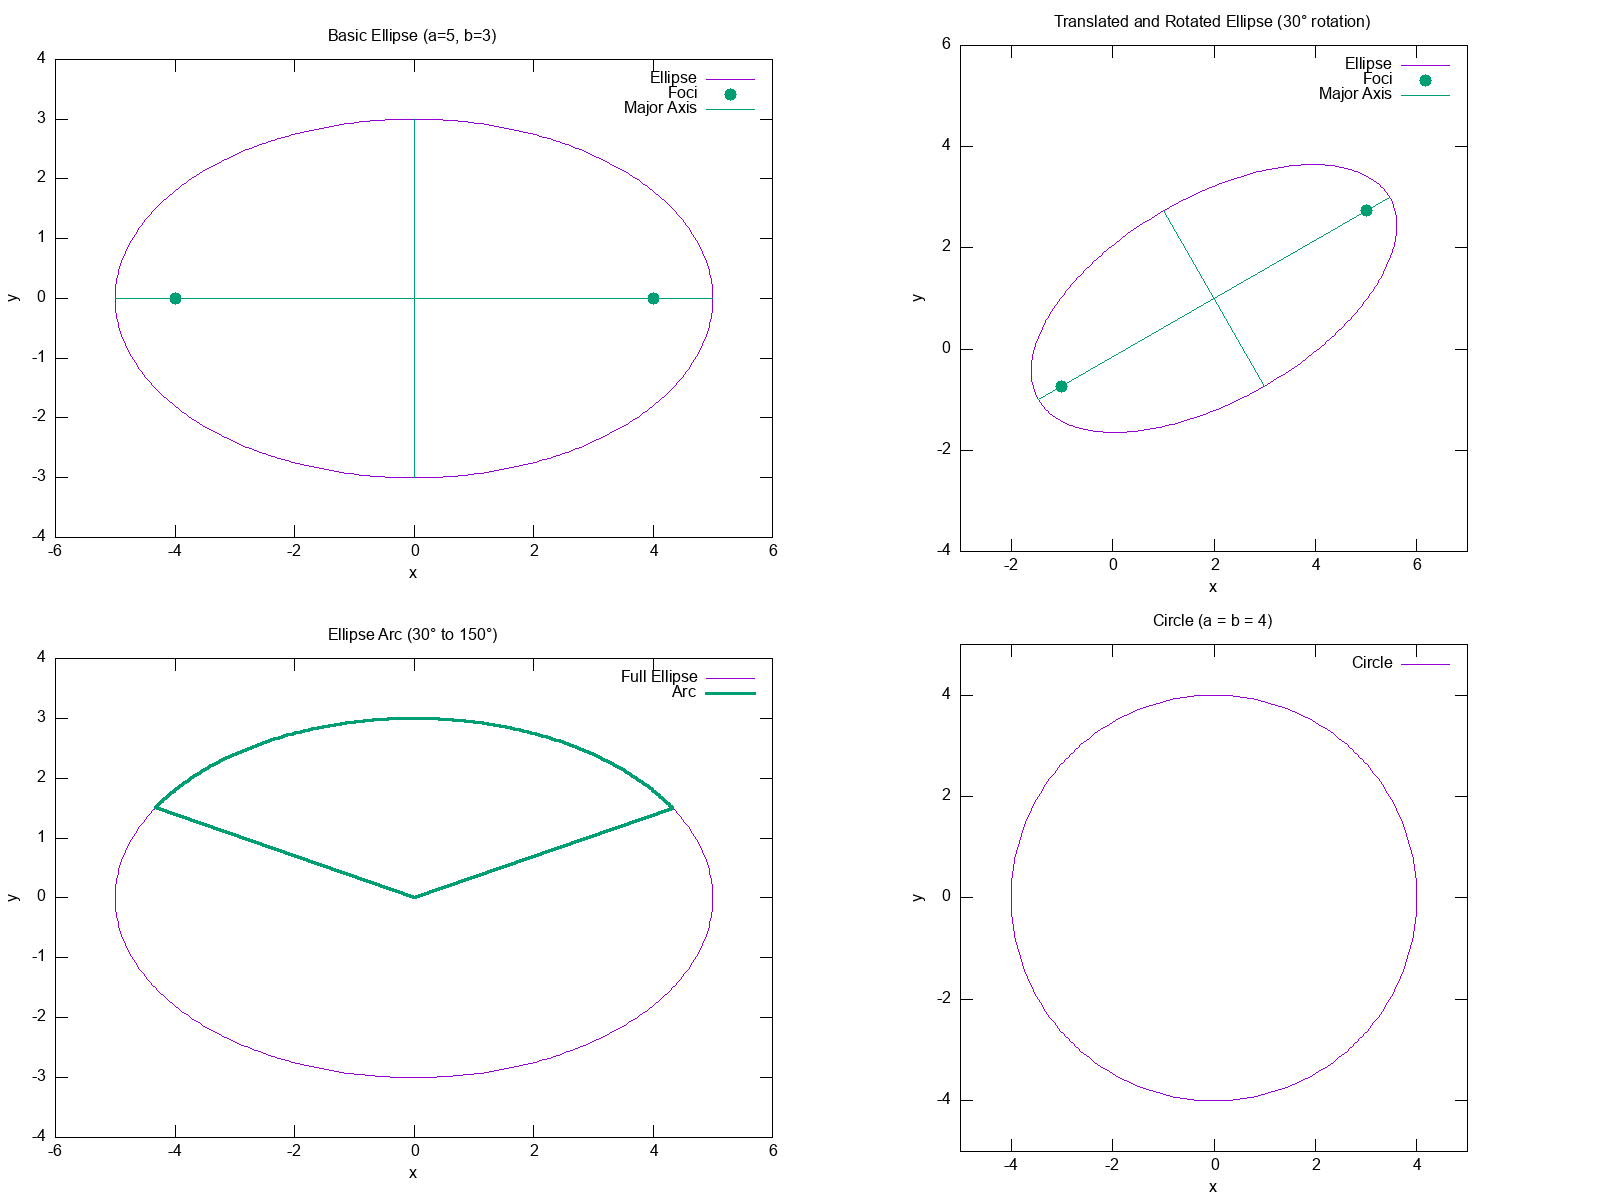
\includegraphics[width=18cm]{ellipse_plots.png}
\end{center}
\caption{ellipse plots}
\end{figure}
}
bash\\
\begin{verbatim}
gcc ellipse_demo.c -o ellipse_demo -lm
./ellipse_demo
\end{verbatim}
\clearpage
\begin{verbatim}
 === ELLIPSE MATHEMATICS LESSON ===

1. DEFINITION:
   An ellipse is the set of all points where the sum of distances
   to two fixed points (foci) is constant.

2. STANDARD EQUATION (center at origin, aligned with axes):
   x^2/a^2 + y^2/b^2 = 1
   where a = semi-major axis, b = semi-minor axis (a >= b > 0)

3. PARAMETRIC EQUATIONS:
   x = a·cos(t), y = b·sin(t) where t in [0, 2pi]

4. ECCENTRICITY:
   e = sqrt(1 - b^2/a^2) where 0 <= e < 1
   e = 0: circle, e → 1: highly elongated ellipse

5. FOCI:
   Located at (±c, 0) where c^2 = a^2 - b^2
   Distance between foci = 2c

6. AREA: A = pi*a*b

7. PERIMETER (approximation):
   P ~= pi[3(a+b) - sqrt((3a+b)(a+3b))] (Ramanujan's formula)

8. TRANSLATION:
   Center at (h,k): (x-h)^2/a^2 + (y-k)^2/b^2 = 1

9. ROTATION:
   Rotate coordinate system by angle theta using rotation matrix

=== Example 1: Basic Ellipse Properties ===
Center: (0.00, 0.00)
Semi-major axis (a): 5.00
Semi-minor axis (b): 3.00
Major axis length: 10.00
Minor axis length: 6.00
Area: 47.12
Perimeter (approx): 25.53
Eccentricity: 0.8000
Foci: (-4.00, 0.00) and (4.00, 0.00)
Focal distance: 8.00

=== Example 2: Translated and Rotated Ellipse ===
Center: (2.00, 1.00)
Semi-axes: a=4.00, b=2.00
Rotation: 30.00°
Area: 25.13
Eccentricity: 0.8660
Foci: (-1.00, -0.73) and (5.00, 2.73)

=== Example 3: Circle (Special Case of Ellipse) ===
When a = b = 4.00, we get a circle
Eccentricity: 0.0000 (0 = perfect circle)
Area: 50.27 (pi*r^2)
Perimeter: 25.13 (2pi*r)

gnuplot script created. Run 'gnuplot plot_ellipse.gp' to generate plots.

Key concepts demonstrated:
- Standard and parametric ellipse equations
- Foci and eccentricity calculation
- Area and perimeter formulas
- Translation and rotation transformations
- Relationship between ellipses and circles
\end{verbatim}

\subsection{ Key Mathematical Concepts Covered:}
\begin{enumerate}
\item \emph{Ellipse Definition}
\begin{quote}
An ellipse is the set of all points where the sum of distances to two fixed points (foci) is constant.                                                                                                      \end{quote}
\item \emph{Standard Equation}
\begin{itemize}
\item Center at origin: \(\frac{x^2}{a^2} + \frac{y^2}{b^2} = 1\) \((a \geq b)\)
\item Translated center: \(\frac{(x-x_c)^2}{a^2} + \frac{(y-y_c)^2}{b^2} = 1\)
\end{itemize}
\item \emph{Parametric Equations}
\begin{itemize}
\item \(x = a\cdot\cos(t)\), \(y = b\cdot\sin(t)\) where \(t \in [0, 2\pi]\)
\item  For rotated ellipses, apply rotation matrix
\end{itemize}

\item \emph{Key Properties}
\begin{itemize}
\item \emph{Semi-major axis (a)}: longest radius
\item \emph{Semi-minor axis (b)}: shortest radius
\item \emph{Eccentricity}: \(e = \sqrt{(1 - b^2/a^2)}\) (\(0 \leq e < 1\))
\item \emph{Foci}: located at distance \(c = \sqrt{(a^2 - b^2)}\) from center
\end{itemize}

\item \emph{Important Formulas}
\begin{itemize}
\item \emph{Area}: A = \(\pi a b\)
\item \emph{Perimeter}: Approximated using Ramanujan's formula
\item \emph{Focal distance}: \( 2c = 2\sqrt{(a^2 - b^2)}\)
\end{itemize}
\item \emph{Special Cases}
\begin{itemize}
\item When \(a = b\): ellipse becomes circle (e = 0)
\item When \(e \rightarrow 1\): ellipse becomes highly elongated
\end{itemize}
\end{enumerate}
The C program demonstrates these concepts with multiple examples and generates gnuplot visualizations showing ellipses with their axes, foci, arcs, and various transformations.\\
An ellipse is the geometric locus of points in a plane for which the sum of the distances from two fixed points F1 and F2, called foci, is constant.\\
An ellipse is a non-degenerate conic section. If we indicate a generic point on the ellipse P, we can translate the definition into the following algebraic condition:\\
\[ PF_1 + PF_2 = constant \]

\begin{thebibliography}{99}
\bibitem{gnuplotJ16} Janert, Philipp K. Gnuplot in action: understanding data with graphs. Simon and Schuster, 2016.
\end{thebibliography}
\end{document}
